\documentclass[12pt]{article}
\usepackage[spanish]{babel} 
\usepackage[utf8]{inputenc}
\usepackage{graphicx} % Incluir imágenes en LaTeX
\usepackage{color} % Para colorear texto
\usepackage{subfigure} % Subfiguras
\usepackage{float} %Posicionamiento [h] en figuras
\usepackage{anysize} % Para personalizar el ancho de  los márgenes

% Para agregar encabezado y pie de página
\usepackage{fancyhdr} 
\pagestyle{fancy}
\fancyhf{}
\fancyhead[L]{\footnotesize Facultad de Ciencias} % Encabezado izquierda
\fancyhead[R]{\footnotesize UNAM}   % Encabezado derecha
\fancyfoot[C]{\thepage}  % Pie centro
\fancyfoot[L]{\footnotesize Inteligencia Artificial}  % Pie izquierda
\renewcommand{\footrulewidth}{0.4pt} % Linea horizontal

\newcommand{\HRule}{\rule{\linewidth}{0.5mm}}

\begin{document}

% ---------------------------------- PORTADA --------------------------------- %

    \begin{center}
        \begin{minipage}{0.48\textwidth} \begin{flushleft}
        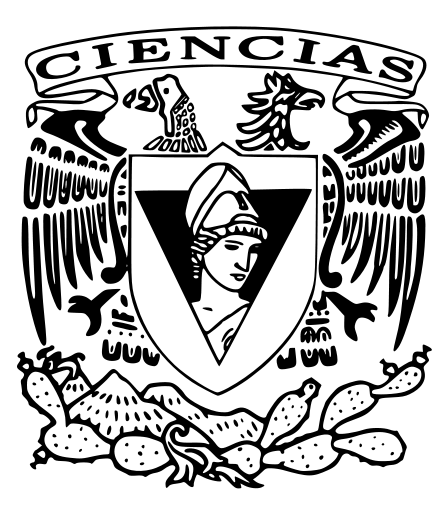
\includegraphics[scale = 0.18]{Images/cnc.png}
        \end{flushleft}\end{minipage}
        \begin{minipage}{0.48\textwidth} \begin{flushright}
        
\includegraphics[scale = 0.25]{Images/nam.png}
        \end{flushright}\end{minipage}

        \vspace*{-1.5cm}

        \textsc{\Large Universidad Nacional \\Autónoma de México}\\[1.5cm]

        \textsc{\LARGE Facultad de Ciencias}\\[3cm]

        \vspace*{.5cm}

        \HRule \\[0.7cm]
        {\Large \bfseries Proyecto Final: Agente que juegue Snake usando redes neuronales}\\[0.4cm]
        \HRule \\[1.5cm]

        \vfill

        \begin{minipage}{0.50\textwidth}
            \begin{center} \large
                \emph{Alumnos:}\\
                Mijail Aron Álvarez Cerrillo
                Alejandro Iabin Arteaga Hernández
                José Fernando Reyes García
                Alejandro Emmanuel Vargas Aldaco
            \end{center}
        \end{minipage}
        %%% % [No quitar] - Espacio para alinear a la izquierda a los asesores %
        \begin{minipage}{0.42\textwidth}
            \begin{center} \large
                \emph{Profesor:} \\
                Gustavo De la Cruz Martínez\\
                \emph{\\Ayudantes:}\\ 
                Estefanía Prieto Larios\\
                Osvaldo Baruch Acevedo Badillo\\
                Rodrígo Eduardo Colín Rivera\\
                
            \end{center}
        \end{minipage}
        \vspace*{1cm}

        \vspace{2cm}
        \begin{center}
            Resumen\\
            {\large 24 de Noviembre, 2019}
        \end{center}                                                             
    \end{center}
    \newpage

    {\bf Introducción}\\
    
        Una de las ramas mas destacadas de la Inteligencia Artificial es la que corresponde a las Redes Neuronales, en el entendido de que son aquellas en cuales existen elementos procesadores de información de cuyas interacciones locales depende el comportamiento del conjunto del sistema.\\
        
        Las redes neuronales tratan de emular el comportamiento del cerebro humano, el cual se caracteriza por el aprendizaje a través de la experiencia y extracción de conocimiento genérico a partir de un conjunto de datos ya conocidos\\
        
        Por lo tanto, podemos decir que las características fundamentales de las redes neuronales son: 
        
        \begin{itemize}
            \item {\bf Aprenden  de  la  experiencia:}  Las  redes neuronales  pueden  modificar  su  comportamiento  como respuesta a su entorno. Dado un conjunto de entradas (quizá con las salidas deseadas),  las  redes neuronales  se  ajustan  para  producir  respuestas  consistentes.  Una  amplia  variedad  de  algoritmos  de  entrenamiento  se  han  desarrollado,  cada  uno  con  sus  propias ventajas e inconvenientes. 
            
            \item {\bf Generalizan  de  ejemplos  anteriores  a  los  ejemplos  nuevos:}  Una  vez  que  la  redes neuronales  esté  entrenada,  la  respuesta  de  la  red  puede  ser,  hasta  un  cierto  punto,  insensible a pequeñas variaciones en las entradas, lo que las hace idóneas para el reconocimiento de patrones. 
            \item {\bf Abstracción  de  la  esencia  de  las  entradas:} Algunas  redes neuronales  son  capaces  de  abstraer  información  de  un  conjunto  de  entradas.  Por  ejemplo,  en  el  caso  de  reconocimiento  de  patrones,  una  red  puede  ser  entrenada  en  una  secuencia  de  patrones  distorsionados  de  una  letra.  Una  vez  que  la  red  sea  correctamente  entrenada   será   capaz   de   producir   un   resultado   correcto   ante   una   entrada   distorsionada, lo que significa que ha sido capaz de aprender algo que nunca había visto.
            \end{itemize}
            
        {\bf Snake}\\
        
        En la década de los 70's fue lanzado al mundo uno de los videojuegos que más alcanzaría popularidad alrededor de todo el mundo, el cual le debe gran audiencia a la marca Nokia, por incluirlo en uno de sus más populares celulares. Se trata de el juego de Snake.\\
        
        El argumento del juego, es simple: Controlas una serpiente que esta encerrada en una celda de $n x m$ cuadros, y dicha serpiente, tiene de ancho 1 cuadro, y se extiende a lo largo en $l$ cuadros, o sea, su tamaño es de $l x 1$ cuadros. Por lo tanto, su desplazamiento es de cuadro por cuadro, avanzando por su cabeza y arrastrando su cola.\\
        
        Dentro de la celda, caerán aleatoriamente manzanas, o algún alimento para dicha serpiente. El objetivo del jugador pues, es conducirla hasta el alimento, procurando evitar que esta choque, ya sea con una pared, o con su propio cuerpo, el cual, aumentara de tamaño en un cuadro, cada vez que sea alimentada.\\
        
        Es un juego de dinámica simple, pero que ha logrado captar la atención de los jugadores, manteniendo su popularidad aún hoy en día.\\
        
        {\bf Objetivo del proyecto}\\
        
        El objetivo de este proyecto a realizar, es simular a un agente que tenga por fin jugar una partida de Snake, intentado que sea lo más parecido al juego que realizaría un ser humano, esto último, se pretende conseguir con el apoyo de redes neuronales.\\
        
        {\bf Descripción del Agente}\\

        El fin de este agente es jugar Snake valiéndose de una red neuronal que este equipo implemente. \\
        
        Para desarrollar una red neuronal para este caso se necesitan usualmente los siguientes 3 pasos: 
        
        \begin{enumerate}
            \item Generación de datos de entrenamiento.
            \item Entrenamiento de la red neuronal.
            \item Pruebas
        \end{enumerate}
        
        Este conjunto de datos se vera representado como una pareja de tuplas, la primera con 7 valores y la segunda con 3, estando en relación de entrada - salida, o sea, la primer tupla es la entrada que se recibe y la segunda es el movimiento que hace dada esa entrada. La estructura de las tuplas esta hecha a fin de representar la información de la siguiente manera.\\
        
        Para los datos de entrada, están representados:
        \begin{enumerate}
            \item Sobre el cuadro que esta a la izquierda de la cabeza, si esa bloqueado o no (1 o 0).
            \item Sobre el cuadro que esta enfrente, si esa bloqueado o no (1 o 0).
            \item Sobre el cuadro que esta a la derecha, si esa bloqueado o no (1 o 0).
            \item Valor $X$ de la posición del alimento de la serpiente.
            \item Valor $Y$ de la posición del alimento de la serpiente.
            \item Valor $X$ de la posición actual de la serpiente (cabeza).
            \item Valor $Y$ de la posición actual de la serpiente (cabeza).
        \end{enumerate}
        La razón por la que se utilizaron estos datos de entrada y no el tablero completo como se había propuesto al principio, es que debido a la enorme complejidad combinatoria del tablero entero, para que la red comenzara a percibir aprendizaje significativo, se necesitaba una enorme cantidad de datos de entrenamiento, y ya que el objetivo final era que simulara el comportamiento humano, necesitábamos una ingente cantidad de datos generados por humanos, lo cual es muy difícil de obtener, creemos que los datos utilizados en la entrada son suficientes para un aprendizaje adecuado sin demasiadas variables\\
        
        Por cuestiones de tiempo y disponibilidad, el conjunto de datos de entrenamiento no se genera por juegos propios de los integrantes del equipo. En su lugar, y para facilitar el desarrollo del conjunto para entrenamiento se tiene un método, que calcula el ángulo entre la posición de la serpiente y el alimento, por lo que le indica cual dirección seguir a fin de llegar al alimento.\\
        
        Para los datos de salida, sencillamente es:
        \begin{enumerate}
            \item (1,0,0) la serpiente gira a la izquierda.
            \item (0,1,0) la serpiente se mantiene en la misma dirección.
            \item (0,0,1) la serpiente gira a la derecha.
        \end{enumerate}
        
        La arquitectura de la red neuronal son 4 capas densas 
        la primera es la capa de entrada con 7 nodos,
        las 2 siguientes son las capas intermedias, cada una con 64 nodos y activación relu.
        Y la última es la capa de salida, consta de 3 neuronas y con activación softmax.\\
        Entrenamos el modelo en nuestras computadoras y solo agregamos el modelo ya entrenado, pero para ver la arquitectura de la red, agregamos también el archivo de python con la red y los archivos de entrenamiento.\\
        
        El modelo queda de la siguiente manera:
        
        \begin{center}
            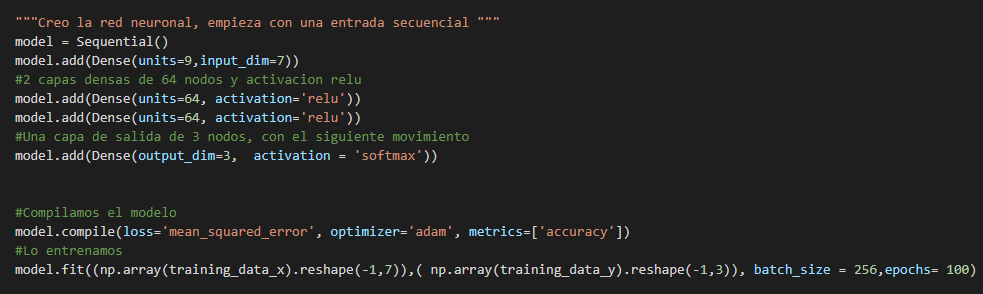
\includegraphics[scale=0.5]{red.PNG}  
        \end{center}
        
        Se hicieron 100 iteraciones de entrenamiento y se utilizó la función adam como función de aprendizaje.
        
        {\bf Tipo de Agente}\\
        
        El tipo de agente ideal para atacar este problema es del tipo que aprende. La forma en que trabaja se puede ver en la siguiente figura: 
        
        \begin{center}
            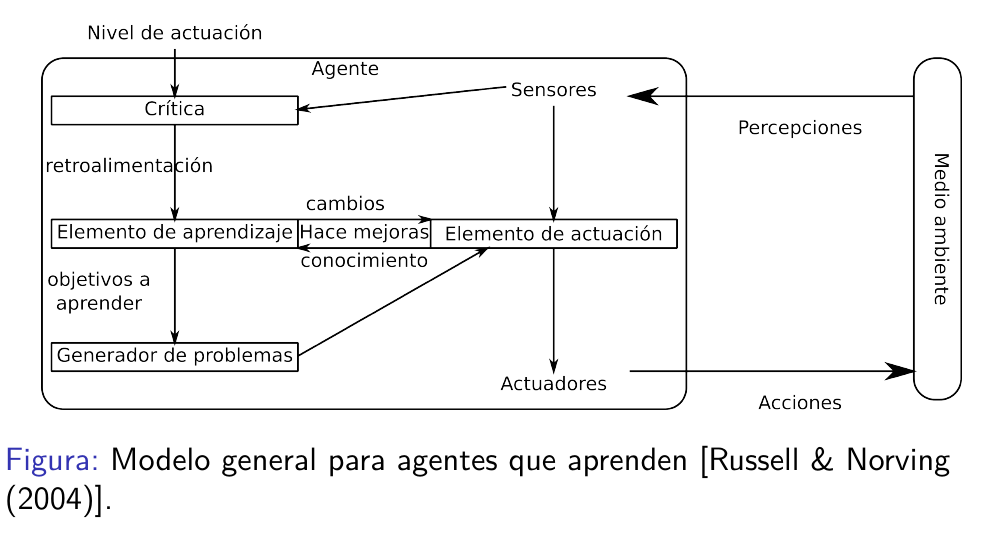
\includegraphics[scale=0.5]{Images/Agente_Aprende.png}  
        \end{center}
        
        Justo el objetivo es que la red neuronal aprenda de cada dato que obtiene como es mejor jugar.\\
        
        {\bf Rendimiento}\\
        
        La medida de rendimiento para determinar la efectividad del agente será el numero de alimentos capaz de tomar antes de chocar y por ende, terminar el juego. O bien, de la misma manera, la longitud de la serpiente al momento de un choque.\\
        
        {\bf Sensores}\\
        
        Los datos de entrada para el agente son los datos previamente mencionados, que van conformando el conjunto de datos de entrenamiento para la red neuronal implementada. Estos datos deben estar cargados previos a una partida. Al momento de jugar, los datos de entrada son su posicion $(x_s, y_s)$, y la posicion del alimento $(x_a, y_a)$\\
        
        {\bf Actuadores}\\
        
        Son las instrucciones de movimiento que hará sobre la serpiente, que son simplemente "Girar izquierda", "Girar derecha" y "Seguir adelante".\\
        
        {\bf Entorno}\\
        
        El entorno en el que trabaja es una celda de $n x m$ cuadros, en los cuales se puede desplazar siempre y cuando no choque con algo. Por lo que se puede afirmar que el entorno es {\bf discreto}. Es de notar que se trata de un único agente que interactúa, por lo que se trata de un {\bf agente individual}\\
        
        Es {\bf parcialmente observable}, pues puede conocer su ubicación en el tablero con vectores de posición $(x, y)$, así como la posición del alimento hacia donde se debe dirigir, pero no tiene noción de donde está la totalidad de su cuerpo.\\
        
        Cada que recolecta algún alimento, el entorno se modifica, pues se agrega otro alimento en otra posición aleatoria. Por lo tanto, es {\bf secuencial}, y dado que se coloca aleatoriamente el alimento, es {\bf estocástico}.\\ \\
        
        En resumen, el REAS para este agente queda modelado de esta forma.
        
        \begin{table}[h]
            \begin{tabular}{|p{1.1cm}|p{4.5cm}|p{2.3cm}|p{2.5cm}|p{2.5cm}|}\hline
            
            Agente & Rendimiento & Entorno & Actuadores & Sensores \\ \hline\hline
            
            Agente que juega Snake  & Longitud de la serpiente hasta el momento de chocar o número de alimentos recolectados antes de choque. & Celda de $n x m$ cuadros, donde uno de ellos tiene un alimento, el cual es el objetivo a conseguir. & Giro a la izquierda, giro a la derecha y seguir adelante &  Dataset de entrenamiento para red neuronal, posiciones de la serpiente y del alimento objetivo. \\ \hline
            \end{tabular}
        \end{table}
        
    {\bf Conclusiones}\\
    
    La red neuronal propuesta, aunque pueda parecer simple, tiene un gran rendimiento, logra imitar de manera muy parecida el comportamiento determinista con el cual fue entrenado, el siguiente paso es generar un dataset que contenga una gran cantidad de juegos humanos, para corroborar su comportamiento con movimientos no deterministas.\\
        
    {\bf Referencias }
    \begin{itemize}
        \item Raquel Flórez López, José Miguel Fernández Fernández, 2008, Las redes neuronales artificiales, Fundamentos teoricos y aplicaciones practicas.
        \item https://es.wikipedia.org/wiki/Red\_neuronal\_artificial
        \item https://www.frro.utn.edu.ar/repositorio/catedras/quimica/5\_anio/
        
        orientadora1/monograias/matich-redesneuronales.pdf
        
        \item Notas de Veronica Esther Arriola Rios
        
        https://sites.google.com/a/ciencias.unam.mx/redesneuronales/apuntes
        
        \item https://theailearner.com/2018/04/19/snake-game-with-deep-learning/
        
    \end{itemize}{}    
    
\end{document}
